\chapter{Maquette}
\label{s:mockup}

\section{Fenêtre principale}

\begin{figure}[H]
	\centering
	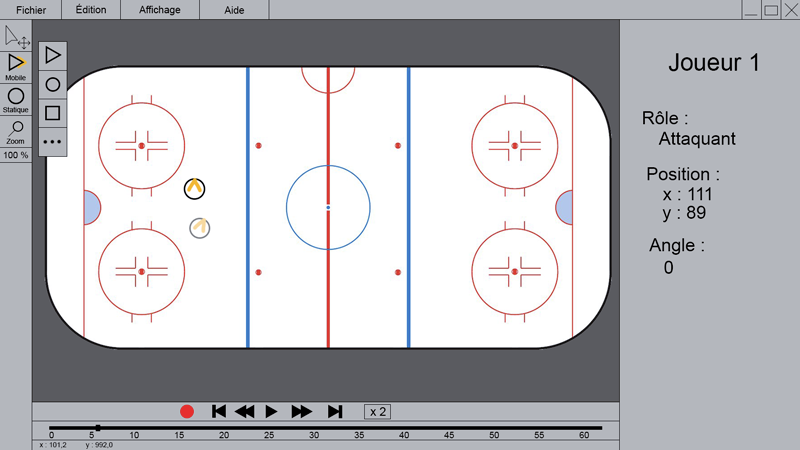
\includegraphics[width=\textwidth]{mockup/mockup.png}
	\caption{Maquette principale de l'application}
	\label{fig:mock-up}
\end{figure}

\subsection{Section du centre}

Cette section est celle où la scène est affichée. Dans le fond de la scène s'affiche le terrain. C'est dans cette section que les éléments sont placés. En plaçant la souris sur un élément, une icône s'affiche. En appuyant dessus, il est possible de modifier l'angle de l'élément.

\subsection{Section de droite}

Cette section contient les paramètres de l'élément actuellement sélectionné. Le premier champ, où il est écrit «~Joueur 1~», est le nom de l'élément. Le «~Attaquant~» est le rôle du joueur. C'est une liste déroulante dans laquelle les valeurs sont celles entrées dans les paramètres du sport. La position en x et en y de l'élément est modifiable via des champs numériques. L'angle est aussi modifiable en utilisant une glissière. Notez qu'il n'y a pas de rôle pour les éléments statiques et les balles, mais que leurs attributs sont tout de même modifiable dans cette interface.

\subsection{Section du bas}

Cette section permet de gérer la visualisation de la stratégie. Le cercle rouge permet de démarrer l'enregistrement de la stratégie. Les autres boutons sont les boutons traditionnels lors du visionnement de vidéo. Le \textit{x2} est dans un champ numérique. En changeant sa valeur, on modifie la vitesse de défilement lors d'avance rapide et de recul. Notez que le «~x~» est seulement présent pour l'affichage. Lorsque l'on édite le champ, il n'est pas présent.

En dessous se trouve une ligne du temps. Le rectangle noir, le curseur, indique quelle image est affichée dans la scène. En le modifiant, l'image affichée dans la scène change. On peut voir juste en dessous la position en x et en y de la souris.

\subsection{Section de gauche}

Cette section contient les boutons permettant d'ajouter des éléments à la scène. C'est la barre d'outils. Le premier à partir du haut est celui utilisé pour déplacer les éléments. Le second sert à créer les éléments mobiles. Le troisième sert à créer les éléments statiques. En maintenant un clic sur le second et le troisième bouton, des icônes apparaissent à droite. Ils permettent de modifier l'élément qui sera ajouté à la scène grâce aux outils d'ajout d'éléments. Le quatrième bouton sert à zoomer sur la scène. Juste en dessous se trouve un champ numérique, permettant de modifier le zoom. La molette de la souris permet aussi de réaliser cette tâche.

\subsection{Menu}

Le menu se retrouve en haut complètement. À l'intérieur de ces menus, on retrouve les commandes pour charger et sauvegarder la stratégie, les commandes qui permettent d'annuler ou de rétablir la dernière action ainsi que différentes options d'affichage. C'est à partir de ce menu que l'on peut charger l'éditeur de sport. La grande majorité de ces commandes ont des raccourcis claviers afin de permettre leur utilisation rapide.

\section{Fenêtre de configuration de sport}

\begin{figure}[H]
	\centering
	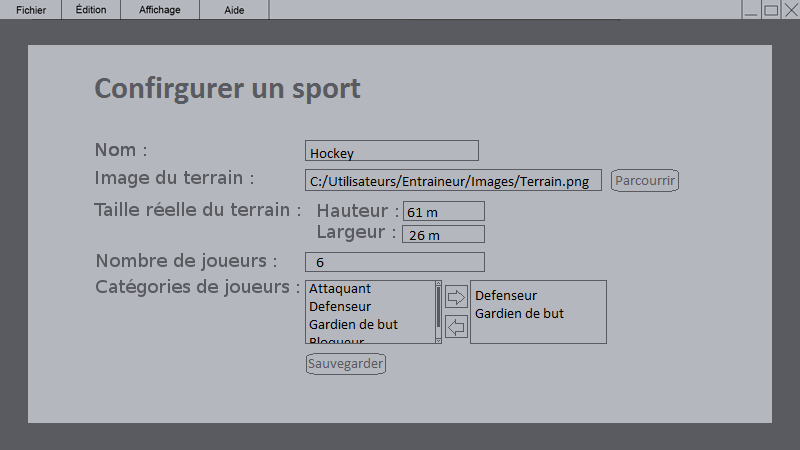
\includegraphics[width=\textwidth]{mockup/mockupSport.png}
	\caption{Maquette de l'écran dde configuration de sport}
	\label{fig:mock-up-sport}
\end{figure}

\subsection{Description}

La figure \ref{fig:mock-up-sport} présente la fenêtre d'édition du sport. Cette fenêtre est accessible via les menus de la fenêtre principale.

Elle est constituée d'un formulaire qui permet d'entrer le nom du sport, de spécifier l'image utilisée comme arrière-plan et les dimensions du terrain. Il permet aussi de modifier le nombre de joueurs et de choisir les rôles des joueurs pouvant faire partie du sport.